\section{La Collecte des données relatives a ce système}

Après avoir délimiter notre projet selon nos besoins et étudier le contexte ainsi que la description des scénarios susceptibles de générer de la valeur. Nous venons ici collecter ces données relatives a ce pays.

Par collecte de données, on entend l'approche systématique qui consiste a réunir et a mesurer des informations en provenance des compteurs, afin d'obtenir une vue complété et précise de la consommation d'énergie. La collecte des données permet aux utilisateurs ou a l'entreprise Sonelgaz de répondre a des questions pertinentes, d'évaluer des résultats et de mieux anticiper les probabilités et les tendances a venir. 

Dans le cadre de notre travail on va classer ces données en deux catégories a savoir:

\textbf{Les données fixes :} Une donnée fixe est en général immuable c'est-a-dire son état ne peut être modifier au fil du temps.

\textbf{Les données évolutives :} On dit qu'une donnée est évolutive si dans un même
contexte, sa valeur change au fil du temps.

Selon notre contexte a étudier, Les données sur lesquelles nous informe ce système sont regroupées dans le tableau suivant :

\begin{figure}[h]
	\centering
	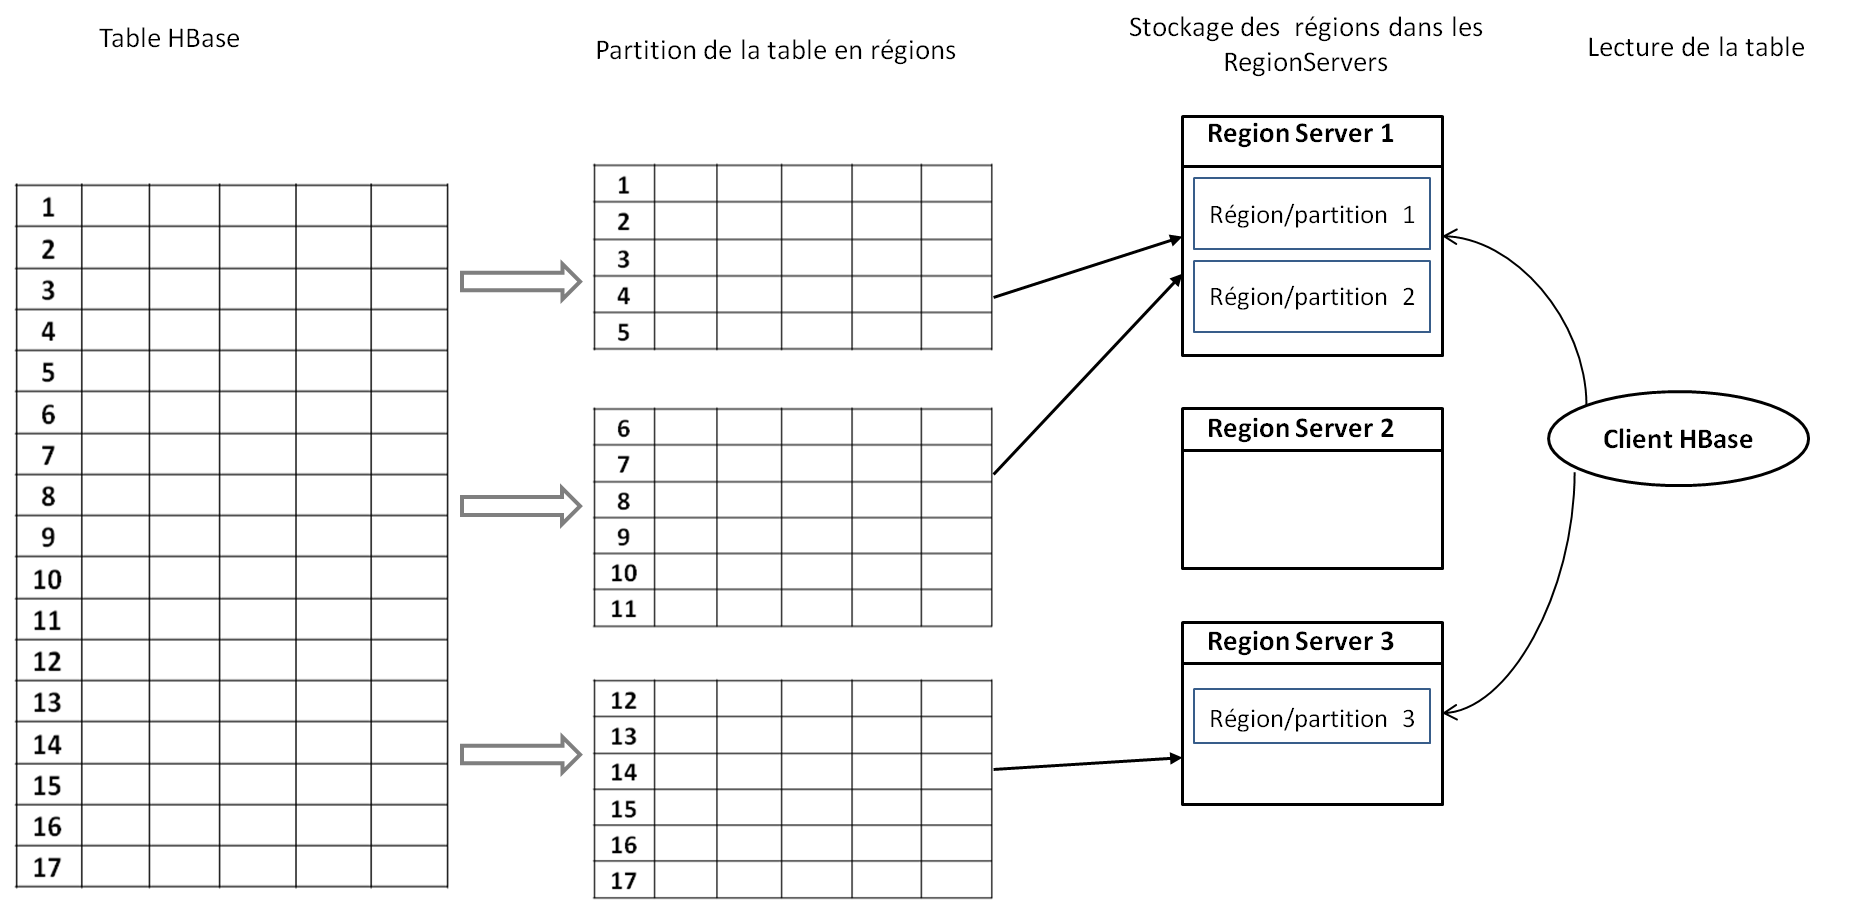
\includegraphics[scale=0.8]{img/part2/2.3.png}
	\caption{Exemple de donnees collectees}
\end{figure}
